% This file was created with tikzplotlib v0.10.1.
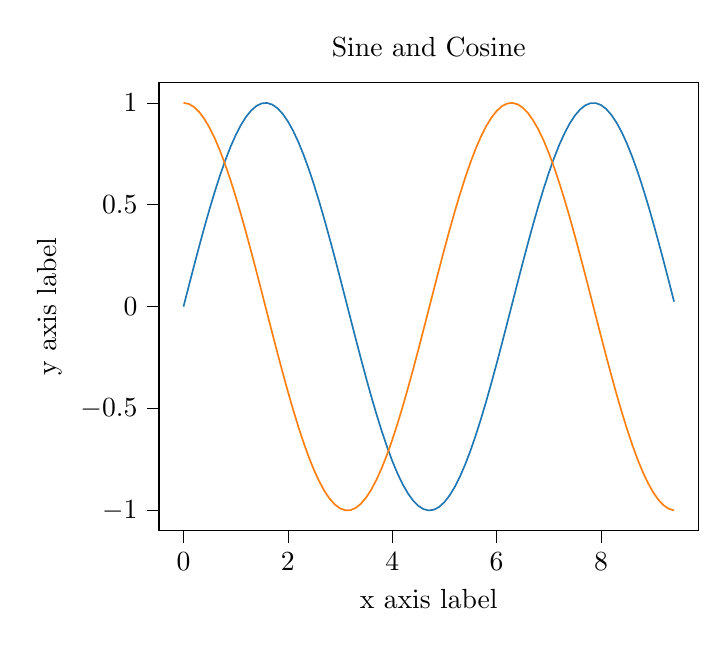
\begin{tikzpicture}

\definecolor{darkgray176}{RGB}{176,176,176}
\definecolor{darkorange25512714}{RGB}{255,127,14}
\definecolor{steelblue31119180}{RGB}{31,119,180}

\begin{axis}[
tick align=outside,
tick pos=left,
title={Sine and Cosine},
x grid style={darkgray176},
xlabel={x axis label},
xmin=-0.47, xmax=9.87,
xtick style={color=black},
y grid style={darkgray176},
ylabel={y axis label},
ymin=-1.09991942044231, ymax=1.09999616287821,
ytick style={color=black}
]
\addplot [semithick, steelblue31119180]
table {%
0 0
0.1 0.0998334166468282
0.2 0.198669330795061
0.3 0.29552020666134
0.4 0.389418342308651
0.5 0.479425538604203
0.6 0.564642473395035
0.7 0.644217687237691
0.8 0.717356090899523
0.9 0.783326909627483
1 0.841470984807897
1.1 0.891207360061435
1.2 0.932039085967226
1.3 0.963558185417193
1.4 0.98544972998846
1.5 0.997494986604054
1.6 0.999573603041505
1.7 0.991664810452469
1.8 0.973847630878195
1.9 0.946300087687414
2 0.909297426825682
2.1 0.863209366648874
2.2 0.80849640381959
2.3 0.74570521217672
2.4 0.675463180551151
2.5 0.598472144103956
2.6 0.515501371821464
2.7 0.42737988023383
2.8 0.334988150155905
2.9 0.239249329213982
3 0.141120008059867
3.1 0.0415806624332905
3.2 -0.0583741434275801
3.3 -0.157745694143249
3.4 -0.255541102026832
3.5 -0.35078322768962
3.6 -0.442520443294852
3.7 -0.529836140908493
3.8 -0.611857890942719
3.9 -0.687766159183974
4 -0.756802495307928
4.1 -0.818277111064411
4.2 -0.871575772413588
4.3 -0.916165936749455
4.4 -0.951602073889516
4.5 -0.977530117665097
4.6 -0.993691003633465
4.7 -0.999923257564101
4.8 -0.996164608835841
4.9 -0.982452612624332
5 -0.958924274663138
5.1 -0.925814682327732
5.2 -0.883454655720153
5.3 -0.832267442223901
5.4 -0.772764487555987
5.5 -0.705540325570392
5.6 -0.631266637872321
5.7 -0.550685542597638
5.8 -0.464602179413757
5.9 -0.373876664830236
6 -0.279415498198926
6.1 -0.182162504272095
6.2 -0.0830894028174964
6.3 0.0168139004843506
6.4 0.116549204850494
6.5 0.215119988087816
6.6 0.311541363513379
6.7 0.404849920616598
6.8 0.494113351138609
6.9 0.5784397643882
7 0.656986598718789
7.1 0.728969040125876
7.2 0.793667863849153
7.3 0.850436620628565
7.4 0.898708095811627
7.5 0.937999976774739
7.6 0.967919672031487
7.7 0.988168233877
7.8 0.998543345374605
7.9 0.998941341839772
8 0.989358246623382
8.1 0.969889810845086
8.2 0.940730556679773
8.3 0.902171833756293
8.4 0.854598908088281
8.5 0.79848711262349
8.6 0.734397097874113
8.7 0.662969230082182
8.8 0.584917192891762
8.9 0.501020856457885
9 0.412118485241757
9.1 0.319098362349352
9.2 0.222889914100246
9.3 0.124454423507062
9.4 0.0247754254533578
};
\addplot [semithick, darkorange25512714]
table {%
0 1
0.1 0.995004165278026
0.2 0.980066577841242
0.3 0.955336489125606
0.4 0.921060994002885
0.5 0.877582561890373
0.6 0.825335614909678
0.7 0.764842187284488
0.8 0.696706709347165
0.9 0.621609968270664
1 0.54030230586814
1.1 0.453596121425577
1.2 0.362357754476673
1.3 0.267498828624587
1.4 0.169967142900241
1.5 0.0707372016677029
1.6 -0.0291995223012888
1.7 -0.128844494295525
1.8 -0.227202094693087
1.9 -0.323289566863504
2 -0.416146836547142
2.1 -0.504846104599858
2.2 -0.588501117255346
2.3 -0.666276021279824
2.4 -0.737393715541246
2.5 -0.801143615546934
2.6 -0.856888753368947
2.7 -0.904072142017061
2.8 -0.942222340668658
2.9 -0.970958165149591
3 -0.989992496600445
3.1 -0.999135150273279
3.2 -0.998294775794753
3.3 -0.987479769908865
3.4 -0.966798192579461
3.5 -0.936456687290796
3.6 -0.896758416334147
3.7 -0.848100031710408
3.8 -0.790967711914417
3.9 -0.72593230420014
4 -0.653643620863612
4.1 -0.574823946533269
4.2 -0.490260821340699
4.3 -0.400799172079975
4.4 -0.307332869978419
4.5 -0.21079579943078
4.6 -0.112152526935054
4.7 -0.0123886634628906
4.8 0.0874989834394473
4.9 0.186512369422576
5 0.283662185463226
5.1 0.377977742712981
5.2 0.468516671300377
5.3 0.554374336179162
5.4 0.634692875942635
5.5 0.70866977429126
5.6 0.77556587851025
5.7 0.83471278483916
5.8 0.885519516941319
5.9 0.927478430744036
6 0.960170286650366
6.1 0.983268438442585
6.2 0.996542097023217
6.3 0.999858636383415
6.4 0.993184918758193
6.5 0.976587625728023
6.6 0.950232591958529
6.7 0.914383148235319
6.8 0.869397490349825
6.9 0.815725100125357
7 0.753902254343305
7.1 0.684546666442806
7.2 0.608351314532255
7.3 0.526077517381105
7.4 0.43854732757439
7.5 0.346635317835026
7.6 0.251259842582255
7.7 0.153373862037864
7.8 0.0539554205626489
7.9 -0.0460021256395369
8 -0.145500033808614
8.1 -0.243544153735791
8.2 -0.339154860983836
8.3 -0.431376844970621
8.4 -0.519288654116686
8.5 -0.602011902684824
8.6 -0.678720047320012
8.7 -0.7486466455974
8.8 -0.811093014061656
8.9 -0.865435209241112
9 -0.911130261884677
9.1 -0.947721602131112
9.2 -0.974843621404164
9.3 -0.992225325452603
9.4 -0.999693042035206
};
\end{axis}

\end{tikzpicture}
